
\documentclass{beamer}
\mode<presentation>
\usepackage{amsmath,amssymb,mathtools}
\usepackage{textcomp}
\usepackage{gensymb}
\usepackage{adjustbox}
\usepackage{subcaption}
\usepackage{enumitem}
\usepackage{multicol}
\usepackage{listings}
\usepackage{url}
\usepackage{graphicx}
\def\UrlBreaks{\do/\do-}

\usetheme{Boadilla}
\usecolortheme{lily}
\setbeamertemplate{footline}{
\leavevmode
\hbox{
\begin{beamercolorbox}[wd=\paperwidth,ht=2ex,dp=1ex,right]{author in head/foot}
\insertframenumber{} / \inserttotalframenumber\hspace*{2ex}
\end{beamercolorbox}}
\vskip0pt
}
\setbeamertemplate{navigation symbols}{}

\lstset{
frame=single,
breaklines=true,
columns=fullflexible,
basicstyle=\ttfamily\tiny
}

\numberwithin{equation}{section}

\newcommand{\myvec}[1]{\ensuremath{\begin{pmatrix}#1\end{pmatrix}}}
\let\vec\mathbf

\title{Matgeo Presentation - Problem 2.5.29}
\author{V.Sainadh -- EE25BTECH11061}

\begin{document}


\begin{frame}

\titlepage

\end{frame}

\begin{frame}{Problem Statement}
The points $\vec{A} = (4,7),\ \vec{B} = (p,3),\ \vec{C} = (7,3)$ are the vertices of a right triangle, 
right-angled at $\vec{B}$. Find the value of $p$.
\end{frame}

\begin{frame}{Solution: Condition for Right Angle at B}

Let
\begin{align}
\vec{A}=\myvec{4\\7},\quad
\vec{B}=\myvec{p\\3},\quad
\vec{C}=\myvec{7\\3}
\end{align}

Right angle at \(\vec{B}\) \(\implies\) the dot product of the adjacent sides at \(\vec{B}\) is zero:
\begin{align}
(\vec{A}-\vec{B})^T(\vec{C}-\vec{B})=0
\end{align}



\end{frame}

\begin{frame}{Solution: }
Compute the vectors:
\begin{align}
\vec{A}-\vec{B}=\myvec{4-p\\4},\qquad
\vec{C}-\vec{B}=\myvec{7-p\\0}
\end{align}

Their dot product:
\begin{align}
(\vec{A}-\vec{B})^T(\vec{C}-\vec{B})
&= \myvec{4-p\\4}^T\myvec{7-p\\0} \\
&= (4-p)(7-p)+4\cdot 0 \\
&= (4-p)(7-p)
\end{align}


\end{frame}

\begin{frame}{Solution: }
    Right angle condition gives:
\begin{align}
(4-p)(7-p)=0 \ \Rightarrow\ p=4\ \text{or}\ p=7
\end{align}

If \(p=7\), then \(\vec{B}=\vec{C}\) (degenerate). Hence,
\begin{align}
\boxed{p=4}
\end{align}

\end{frame}

\begin{frame}{Result Plot}
\begin{figure}[H]
\centering
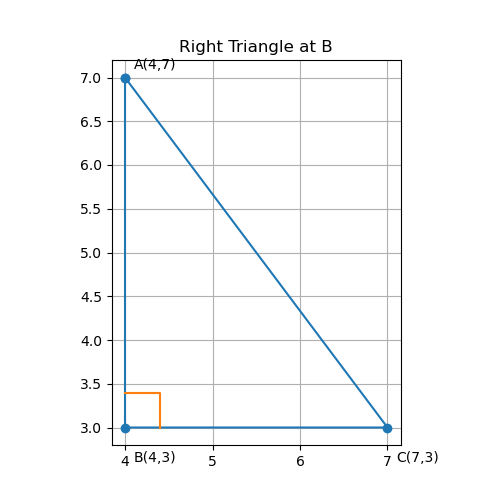
\includegraphics[width=0.7\columnwidth]{figs/Figure_1.png}
\caption*{Right Triangle at \vec{B}}
\end{figure}

\end{frame}


\begin{frame}[fragile]{C Source Code: points.c}
\begin{lstlisting}[language=C]
// geom.c
#include <stdio.h>

int is_right_at_B(int Ax, int Ay, int Bx, int By, int Cx, int Cy) {
    long BAx = Ax - Bx, BAy = Ay - By;
    long BCx = Cx - Bx, BCy = Cy - By;
    long dot = BAx * BCx + BAy * BCy;
    return dot == 0 ? 1 : 0;
}

int solve_p_for_given_question(void) {
    // A(4,7), B(p,3), C(7,3); right angle at B ⇒ (4-p,4)·(7-p,0)=0 ⇒ p=4
    return 4;
}

\end{lstlisting}

\end{frame}

\begin{frame}[fragile]{Python Script: call c.py}
\begin{lstlisting}[language=Python]
# use_geom.py
import ctypes
from ctypes import c_int

lib = ctypes.CDLL("./libgeom.so")

lib.is_right_at_B.argtypes = [c_int, c_int, c_int, c_int, c_int, c_int]
lib.is_right_at_B.restype  = c_int

lib.solve_p_for_given_question.argtypes = []
lib.solve_p_for_given_question.restype  = c_int

p = lib.solve_p_for_given_question()
print(p)

ok = lib.is_right_at_B(4, 7, p, 3, 7, 3)
print("RIGHT" if ok else "NOT_RIGHT")

\end{lstlisting}
\end{frame}



\begin{frame}[fragile]{Python Script: plot.py}
\begin{lstlisting}[language=Python]
# triangle_plot.py
# Plot A(4,7), B(p,3), C(7,3) with p=4 (right angle at B)

import math
import matplotlib.pyplot as plt

# Points
A = (4, 7)
p = 4
B = (p, 3)
C = (7, 3)

# Unpack for plotting
xs = [A[0], B[0], C[0], A[0]]
ys = [A[1], B[1], C[1], A[1]]

# Draw triangle
plt.figure(figsize=(5, 5))
plt.plot(xs, ys, marker='o')

# Labels
plt.text(A[0]+0.1, A[1]+0.1, "A(4,7)")
plt.text(B[0]+0.1, B[1]-0.4, f"B({p},3)")
plt.text(C[0]+0.1, C[1]-0.4, "C(7,3)")
\end{lstlisting}
\end{frame}

\begin{frame}[fragile]{Python Script: plot.py}
\begin{lstlisting}[language=Python]
# Indicate right angle at B by plotting little square
# Vector BA and BC
BA = (A[0]-B[0], A[1]-B[1])
BC = (C[0]-B[0], C[1]-B[1])
# Small step along each to draw the corner
scale = 0.4
p1 = (B[0] + scale * (BA[0]/math.hypot(*BA)), B[1] + scale * (BA[1]/math.hypot(*BA)))
p2 = (B[0] + scale * (BC[0]/math.hypot(*BC)), B[1] + scale * (BC[1]/math.hypot(*BC)))
corner = (p1[0] + (p2[0]-B[0]), p1[1] + (p2[1]-B[1]))
plt.plot([p1[0], corner[0], p2[0]], [p1[1], corner[1], p2[1]])

plt.gca().set_aspect('equal', adjustable='box')
plt.grid(True)
plt.title("Right Triangle at B")

# Always save to a file so you have output even without a display
plt.savefig("triangle.png", dpi=150)



\end{lstlisting}
\end{frame}



\end{document}
